\documentclass[a4paper,twoside]{report} % for a report (default)

\usepackage{amsmath}
\usepackage{bftn} % You need this
\usepackage{cite}
\usepackage{color}
\usepackage{listings}

\title{Inter-dispatcher communication in Barrelfish}   % title of report
\author{Andrew Baumann}	% author
\tnnumber{011}  % give the number of the tech report
\tnkey{IDC} % Short title, will appear in footer

% \date{Month Year} % Not needed - will be taken from version history

\begin{document}
\maketitle

%
% Include version history first
%
\begin{versionhistory}
\vhEntry{0.0}{06.08.2010}{AB}{Initial version}
\vhEntry{0.1}{01.09.2010}{AB}{Documented Flounder IDL, stub API and waitset}
\vhEntry{0.2}{21.10.2010}{AB}{Completed runtime support chapter}
\vhEntry{0.3}{05.12.2011}{MN}{Added meta-parameter note, AHCI references}
\end{versionhistory}

% \intro{Abstract}		% Insert abstract here
% \intro{Acknowledgements}	% Uncomment (if needed) for acknowledgements
% \tableofcontents		% Uncomment (if needed) for final draft
% \listoffigures		% Uncomment (if needed) for final draft
% \listoftables			% Uncomment (if needed) for final draft

\lstset{
  language=C,
  basicstyle=\ttfamily \small,
  flexiblecolumns=false,
  basewidth={0.5em,0.45em},
  boxpos=t,
}

\newcommand{\note}[1]{[\textcolor{red}{\emph{#1}}]}

\tableofcontents

%%%%%%%%%%%%%%%%%%%%%%%%%%%%%%%%%%%%%%%%%%%%%%%%%%%%%%%%%%%%%%%%%%%%%%%%
\chapter{Introduction}

TODO

\chapter{Flounder stub compiler}\label{cha:flounder}

\section{Overview}

\section{Interface definition language}\label{sec:idl}

\subsection{Lexical conventions}
The following convention, derived from Mackerel\cite{btn002-mackerel} has
been adopted for Flounder. It is similar to the convention in modern
day programming languages like C and Java.

\begin{description}
\item[Whitespace:]  As in C and Java, Flounder considers sequences of
  space, newline, tab, and carriage return characters to be
  whitespace.  Whitespace is generally not significant. 

\item[Comments:] Flounder supports C-style comments.  Single line comments
  start with \texttt{//} and continue until the end of the line.
  Multiline comments are enclosed between \texttt{/*} and \texttt{*/};
  anything inbetween is ignored and treated as white space.

\item[Identifiers:] Valid Flounder identifiers are sequences of numbers
  (0-9), letters (a-z, A-Z) and the underscore character ``\texttt{\_}''.  They
  must start with a letter or ``\texttt{\_}''.
  \begin{align*}
    identifier & \rightarrow ( letter \mid \_ ) (letter \mid digit \mid \_) \\
    letter & \rightarrow (\textsf{A \ldots Z} \mid  \textsf{a \ldots z})\\
    digit & \rightarrow (\textsf{0 \ldots 9})
\end{align*}
  
\item[Integer Literals:] A Flounder integer literals is a sequence of
  digits, optionally preceded by a radix specifier.  As in C, decimal (base 10)
  literals have no specifier and hexadecimal literals start with
  \texttt{0x}.
\begin{align*}
digit & \rightarrow (\textsf{0 \ldots 9})\\
hexadecimal & \rightarrow (\textsf{0x})(\textsf{0 \ldots 9} \mid \textsf{A
\ldots F} \mid \textsf{a \ldots f})
\end{align*}


\item[Reserved words:] The following are reserved words in Flounder:
\begin{alltt}\begin{tabbing}
xxxxxxxxx \= xxxxxxxxx \= xxxxxxxxx \= xxxxxxxxx \= xxxxxxxxx \= xxxxxxxxx \kill
alias \> call \> enum \> in \> interface \> message \\
out \> response \> rpc \> struct \> typedef 
\end{tabbing}\end{alltt}

\item[Builtin types:] The following identifiers are recognised as builtin types:
\begin{alltt}\begin{tabbing}
xxxxxxxxxxxx \= xxxxxxxxxxxx \= xxxxxxxxxxxx \= xxxxxxxxxxxx \= xxxxxxxxxxxx \=
xxxxxxxxxxxx \kill
bool \> cap \> char \> give_away_cap \> int \> int8 \\
int16 \> int32 \> int64 \> intptr \> iref \> size \\
string \> uint8 \> uint16 \> uint32 \> uint64 \> uintptr
\end{tabbing}\end{alltt}

\item[Special characters:] The following characters are used as operators,
  separators, terminators or for other special purposes in Flounder:
\begin{alltt}
  \{ \} [ ] ( ) ; ,
\end{alltt}

\end{description}


\subsection{Interface specification}

A Flounder input file must specify a single interface, of the form:

\begin{syntax}
interface \synit{name} ["\synit{description}"]
\verb+{+
  \synit{types};
  \ldots
  \synit{messages};
  \ldots
\verb+}+;
\end{syntax}

\begin{description}
\item[name] is an identifier for the interface type, and will be used to
  generate identifiers in the target language (typically C).  While
  not currently enforced by the Flounder compiler, by
  convention this should only differ from the name of the file in case
  and suffix, e.g.\ the file \texttt{xapic.dev} defines a device type
  of name \texttt{xAPIC}. 

\item[description] is a string literal in double quotes, which
  describes the interface being specified, for example
  \texttt{"Name service"}.
\end{description}

After the description string follows in curly brackets a series of
declarations which specify types, messages and their arguments.   Each
declaration must be one of the following:

\begin{itemize}

  \item A transparent type alias, using the \texttt{alias} declaration,
    described in Section~\ref{sec:lang:alias}.

  \item A type definition, using the \texttt{typedef} declaration,
    described in Section~\ref{sec:lang:typedef}.

  \item A simple message specification, using either the \texttt{message},
    \texttt{call} or \texttt{response} declarations, describing a
    single unidirectional message with typed arguments,
    and described in Section~\ref{sec:lang:message}.

  \item An \texttt{rpc} specification, which describes two related
    messages (a call and the response) with a single declaration,
    and described in Section~\ref{sec:lang:rpc}.

\end{itemize}

Type aliases and definitions (\texttt{alias} and \texttt{typedef}) are
optional, but if present must precede all messages. There must be at least
one message in every interface.

\subsection{Transparent type alias}\label{sec:lang:alias}

\begin{syntax}
alias \synit{aliasname} \synit{builtintype};
\end{syntax}

This simply declares a given alias name that may henceforth be used in the
interface file in place of the given builtin type. It does not alter the
generated code.

\subsection{Type definition}\label{sec:lang:typedef}

In contrast to an alias, the \texttt{typedef} keyword causes a new type
to be created in the context of both the interface file and the programming
language where the generated stubs are used.

\subsubsection{Structure}

\begin{syntax}
typedef struct \verb+{+
  \synit{typename} \synit{fieldname};
  \ldots
\verb+}+ \synit{structname};
\end{syntax}

This declares a compound type, akin to a structure in C.

\subsubsection{Fixed-size array}

\begin{syntax}
typedef \synit{typename} \synit{arrayname}\verb+[+\synit{size}\verb+]+;
\end{syntax}

Where \emph{typename} is a previously-defined type, and \emph{size} is an
integer literal, defines an array type with the given \emph{arrayname}. This
name refers to an array of a fixed size.

\subsubsection{Enumeration}

\begin{syntax}
typedef enum \verb+{+
  \synit{fieldname},
  \ldots
\verb+}+ \synit{structname};
\end{syntax}

An enumeration, as in C, is represented as an integer type that may take
one of the predefined symbolic values.

\subsubsection{Alias}

\begin{syntax}
typedef \synit{aliasname} \synit{typename};
\end{syntax}

This form creates a new name (in both Flounder and C) for a
previously-defined or builtin type.


\subsection{Simple message}\label{sec:lang:message}

A simple message specification takes the form:

\begin{syntax}
@\synit{context}\verb+(+\synit{name}\verb+=+\synit{value}, \ldots \verb+)+ \synit{(optional)}
message|call|response \synit{name} \verb+(+\synit{argdecl}, \ldots \verb+)+;
\end{syntax}

The three identifiers \texttt{message}, \texttt{call}, and \texttt{response}
exist for legacy reasons, and are treated identically by the stub compiler.
They may be used as a simple form of documentation, when messages are intended
to travel in a particular direction between client and server.

The meta-parameters beginning with the context identifier are optional and may
be used by individual stub compilers for additional information about messages
that is not part of the payload. Multiple such contexts may also be provided.

Message arguments use a comma-separated C-like syntax, and may take one of the
following forms:

\begin{description}
 \item[Simple arguments] are denoted by type name and argument name literals,
separated by whitespace.
 \item[Dynamic array arguments] include the type name, argument name, and size
name literals, as follows:
\begin{syntax}
\synit{typename} \synit{argname}\verb+[+\synit{sizename}\verb+]+
\end{syntax}
\end{description}

For example, the following defines a message named ``dummy'' with three
arguments: an integer, a character string, and a dynamic array of unsigned 8-bit
integers (ie. a data buffer).

\begin{example}
  message dummy(int32 arg, string s, uint8 buf[buflen]);
\end{example}

\subsection{RPC}\label{sec:lang:rpc}

\begin{syntax}
@\synit{context}\verb+(+\synit{name}\verb+=+\synit{value}, \ldots \verb+)+ \synit{(optional)}
rpc \synit{name} \verb+(+in|out \synit{argdecl}, \ldots \verb+)+;
\end{syntax}

An \texttt{rpc} declaration defines a pair of related one-way messages for the
RPC \emph{call} and its \emph{response}. Argument declarations take the same
syntax as for a simple message, but are prefixed with either \texttt{in} or
\texttt{out}. All \texttt{in} arguments are arguments of the call, and all
\texttt{out} arguments are arguments of the response.

For example, the following defines an RPC that takes as input a string
and returns an \texttt{errval} type (which must previously have been defined):

\begin{example}
  rpc testrpc(in string s, out errval reterr);
\end{example}

With the exception of its special treatment by the RPC client backend
(described in Section~\ref{sec:rpcclient}), this RPC is exactly equivalent
to the following message specifications:

\begin{example}
  message testrpc_call(string s);
  message testrpc_response(errval reterr);
\end{example}

\section{Invocation}

When invoked, Flounder processes a single interface file, and generates into a
single output file the results of one or more \emph{backends}. The names of the
input and output files and the backends to use are determined by the
command-line arguments, which are as follows:

\begin{verbatim}
Usage: flounder [OPTION...] input.if output
  -G       --generic-header    Create a generic header file
           --generic-stub      Create generic part of stub implemention
  -a ARCH  --arch=ARCH         Architecture for stubs
  -i FILE  --import=FILE       Include a given file before processing
           --lmp-header        Create a header file for LMP
           --lmp-stub          Create a stub file for LMP
           --ump-header        Create a header file for UMP
           --ump-stub          Create a stub file for UMP
           --rck-header        Create a header file for RCK
           --rck-stub          Create a stub file for RCK
           --bmp-header        Create a header file for BMP
           --bmp-stub          Create a stub file for BMP
           --loopback-header   Create a header file for loopback
           --loopback-stub     Create a stub file for loopback
           --rpcclient-header  Create a header file for RPC
           --rpcclient-stub    Create a stub file for RPC
           --msgbuf-header     Create a header file for message buffers
           --msgbuf-stub       Create a stub file for message buffers
  -T       --thc-header        Create a THC header file
  -B       --thc-stubs         Create a THC stubs C file
           --ahci-header       Create a header file for AHCI
           --ahci-stub         Create a stub file for AHCI
\end{verbatim}

Zero or more files may be specified as \emph{imports}. An import file
provides a simplistic mechanism for sharing type definitions among multiple
interfaces: it consists of one or more \texttt{alias} or \texttt{typedef}
statements. All import files are processed in the order in which they occur on
the command line, before parsing of the interface definition file begins.
Otherwise, types defined in import files are equivalent to types appearing in
an interface definition.

The architecture option must be specified when generating stubs for either LMP,
UMP, or RCK backends; when specified, it must be one of the architectures
Flounder understands (see \texttt{Arch.hs} in the flounder source), which is
typically the same as the set of architectures supported by Barrelfish.

All other options cause Flounder to emit the C code generated by one of its
backends. The \emph{generic} backend defines the common interface and support
code that is shared by all other backends, and is always required.
Chapter~\ref{cha:hake} describes the location and contents of the generated
files that are used in the Barrelfish build system.

\chapter{Flounder stub API}

Most Flounder backends generate message stubs for specific interconnect
drivers, with implementations varying widely according to the properties of
the interconnect driver. However, common to all interconnect drivers for a
given interface is the interface to the \emph{binding object}, which allows
the typed messages defined in the interface definition to be sent and received
in an event-driven programming style. The interface to the binding object for
a given interface is generated by the \texttt{--generic-header} option to
Flounder, and is documented here.

Most interaction with bindings involves interface-type-specific functions.
In the examples that follow, we assume that a Flounder interface
named \texttt{iface} is used, with the following specification:

\begin{example}
interface iface \{
  message basic(uint32 arg);
  message str(uint32 arg, string s);
  message caps(uint32 arg, cap cap1, cap cap2);
  message buf(uint8 buf[buflen]);
\};
\end{example}


\section{Binding process}\label{sec:binding_bindingproc}

In order to communicate, two dispatchers must establish a communication channel
using a common interconnect driver, and must acquire binding objects for each
endpoint of the channel. This process is known as \emph{binding}, and operates
in two modes:

\begin{enumerate}
 \item A \emph{client} dispatcher initiates a binding to a service by calling
       the interface's \emph{bind} function
 \item A \emph{server} dispatcher accepts an incoming binding request from a
       client, on a service which it has previously \emph{exported}
\end{enumerate}

In any binding attempt, one dispatcher must act as server and the other as
the client, however once a binding is established, the binding objects and the
process of communication on both sides of the binding are equivalent and
indistinguishable.

\subsection{Server-side: export}

In order to accept binding requests, a dispatcher must first export a service.
This is done by calling the \emph{export} function for the given interface:

\begin{lstlisting}
typedef void idc_export_callback_fn(void *st, errval_t err, iref_t iref);
typedef errval_t iface_connect_fn(void *st, struct iface_binding *binding);

errval_t iface_export(void *st, idc_export_callback_fn *export_cb,
                      iface_connect_fn *connect_cb, struct waitset *ws,
                      idc_export_flags_t flags);
\end{lstlisting}

The \lstinline+iface_export()+ function initiates the export of a new service.
It takes a state pointer, export callback, connection callback, waitset
pointer, and flags. If it returns success, the export has been successfully
initiated.

When the export either succeeds or fails, the export callback will be invoked. 
It takes the state pointer (which was passed to \lstinline+iface_export()+), an
error code indicating success or failure of the export, and an \emph{interface
reference} (iref). The iref is only meaningful if the export succeeds; if this
is the case, it identifies the exported service in such a way that a client can
use the iref to initiate a binding to the service. In order for the service to
be usable, the iref must be communicated to the potential clients in some
manner; typically by registering it in the name service, which is described in
Chapter~\ref{cha:nameservice}.

Once a service has been exported, clients may attempt to bind to it. When this
occurs, the connection callback will be invoked. This function takes the state
pointer used at export time, and a pointer to the new partly-constructed binding
object. If it returns success, the binding request will be accepted, and the
binding process will complete. If it returns an error code indicating failure,
the binding attempt will be rejected, and the error code will be returned to
the client. When accepting a binding request, the connection callback also has
the task of filling in the vtable of receive handers, as described in
Section~\ref{sec:binding_rx}, and the error handler, described in
Section~\ref{sec:binding_errors}.

\subsection{Client-side: bind}

In order to initiate a binding, a client dispatcher calls the \emph{bind}
function for a given interface:

\begin{lstlisting}
typedef void iface_bind_continuation_fn(void *st, errval_t err,
                                        struct iface_binding *binding);

errval_t iface_bind(iref_t i, iface_bind_continuation_fn *continuation,
                    void *st, struct waitset *waitset, idc_bind_flags_t flags);
\end{lstlisting}

This function takes the iref for the service (obtained, for example, by a name
service query), a bind continuation function, state pointer, waitset poitner,
and flags. If it returns success, a binding attempt has been initiated.

At some later time, when the binding either completes or fails, the bind
continuation function will be run. This takes the state pointer passed to
\lstinline+iface_bind()+, an error code indicating success or failure, and a
pointer to the newly-constructed binding, which is only valid if the error code
indicates success.

\section{Binding objects}\label{sec:binding_objs}

The end result of the binding process (either client-side or server-side) is a
binding object, which is the abstract interface to a specific interconnect
driver for a specific interface type. It is implemented in C as the
\lstinline+struct iface_binding+ type, the defined portion of which is shown
below, and described in the following sections:

\begin{lstlisting}
struct iface_binding {
    /* Arbitrary user state pointer */
    void *st;

    /* Waitset used for receive handlers and send continuations */
    struct waitset *waitset;

    /* Mutex for the use of user code. */
    /* Must be held before any operation where there is a possibility of
     * concurrent access to the same binding (eg. multiple threads, or
     * asynchronous event handlers that use the same binding object). */
    struct event_mutex mutex;

    /* returns true iff a message could currently be accepted by the binding */
    iface_can_send_fn *can_send;

    /* register an event for when a message is likely to be able to be sent */
    iface_register_send_fn *register_send;

    /* change the waitset used by a binding */
    iface_change_waitset_fn *change_waitset;

    /* perform control operations */
    iface_control_fn *control;

    /* error handler for any async errors associated with this binding */
    /* must be filled-in by user */
    iface_error_handler_fn *error_handler;

    /* Incoming message handlers (filled in by user) */
    struct iface_rx_vtbl rx_vtbl;
};
\end{lstlisting}

The \lstinline+st+ pointer is available for users to associate arbitrary local
state with each binding object. It is not used by the binding implementation.

The \lstinline+waitset+ pointer identifies the waitset used by the binding for
executing receive handler functions, send continuations, and internal logic. It
is read-only for users of the binding; to change the actual waitset, the
\lstinline+change_waitset()+ control function must be used.

Binding implementations are not thread-safe, and it is the responsibility of
user code to ensure that no concurrent access to the same binding occurs.
The \lstinline+mutex+ field is not used by the binding implementation, but is
provided for user code to ensure safety of concurrent accesses to the binding
object. It is used, for example, to arbitrate access to the shared monitor
binding, as described in Section~\ref{sec:monitor}.

The remaining fields are documented in the following sections.


\section{Receiving messages}\label{sec:binding_rx}

When a message arrives, the binding implementation calls the \emph{receive
handler} function located in the binding's \lstinline+rx_vtbl+ table of function
pointers. This table has an entry for each message type, with arguments
corresponding to those of the message, as shown below:

\begin{lstlisting}
/*
 * Message type signatures (receive)
 */
typedef void iface_basic__rx_method_fn(struct iface_binding *_binding, uint32_t arg);
typedef void iface_str__rx_method_fn(struct iface_binding *_binding, uint32_t arg, char *s);
typedef void iface_caps__rx_method_fn(struct iface_binding *_binding, uint32_t arg,
                                      struct capref cap1, struct capref cap2);
typedef void iface_buf__rx_method_fn(struct iface_binding *_binding, uint8_t *buf, size_t buflen);

/*
 * VTable struct definition for the interface (receive)
 */
struct iface_rx_vtbl {
    iface_basic__rx_method_fn *basic;
    iface_str__rx_method_fn *str;
    iface_caps__rx_method_fn *caps;
    iface_buf__rx_method_fn *buf;
};
\end{lstlisting}

It is the responsibility of the user to fill in the \lstinline+rx_vtbl+ when
the binding is initialised, either in the connection callback on the
server side, or in the bind callback on the client side. This is typically
achieved by copying a static table of function pointers. It is a fatal error
if a message arrives on a binding and the handler function for that message
type is uninitialised or NULL.

Any message arguments passed by reference become the property of the user, and
must be freed by the appropriate memory management mechanisms:

\begin{itemize}
 \item Strings and arrays live on the heap, and should be
    released by a call to \lstinline+free()+
 \item Capabilities refer to an occupied capability slot allocated from the
    standard capability space allocator, and should be released by a call to
    \lstinline+cap_destroy()+
\end{itemize}


\section{Sending messages}

A message may be sent on the binding by calling the appropriate transmit
function. For our example interface, these are as follows:

\begin{lstlisting}
errval_t iface_basic__tx(struct iface_binding *_binding, struct event_closure _continuation,
                         uint32_t arg);
errval_t iface_str__tx(struct iface_binding *_binding, struct event_closure _continuation,
                       uint32_t arg, const char *s);
errval_t iface_caps__tx(struct iface_binding *_binding, struct event_closure _continuation,
                        uint32_t arg, struct capref cap1, struct capref cap2);
errval_t iface_buf__tx(struct iface_binding *_binding, struct event_closure _continuation,
                       const uint8_t *buf, size_t buflen);
\end{lstlisting}

Each function takes as arguments the binding pointer and a
\emph{continuation} closure (described below), followed by the message payload.
If it returns success, the message has been successfully enqueued for
transmission, and will eventually be sent if no asynchronous errors occur.

The continuation is optional. When specified, it provides a generic closure
which will be executed after the given message has been successfully sent.
Two macros are provided to construct continuations: \lstinline+NOP_CONT+
provides a no-op continuation, to be used when this functionality is not
required, whereas \lstinline+MKCONT(func,arg)+ constructs a one-off continuation
given a function pointer and its argument.

All binding implementations can buffer exactly one outgoing message. If another
send function is called on the same binding while the buffer is full, the
\lstinline+FLOUNDER_ERR_TX_BUSY+ error will be returned, indicating that the
binding is not currently able to accept another message. In this case, the user
must arrange to retry the send at a later time, typically from a send
continuation function, or by using the \lstinline+register_send()+ control
function (described below).

Any message arguments passed by reference (strings, arrays, and capabilities)
are borrowed by the binding, and must remain live for as long as the message
is buffered but not yet completely sent. The send continuation may be used to
determine when it is safe to reclaim the memory used by reference parameters.


\section{Control functions}

Four standard control functions are defined for all binding implementations,
and are invoked through function pointers in the binding object:
\lstinline+can_send+, \lstinline+register_send+, \lstinline+change_waitset+
and \lstinline+control+.

\subsubsection*{can\_send}

\begin{lstlisting}
typedef bool iface_can_send_fn(struct iface_binding *binding);
\end{lstlisting}

This function returns true if and only if the binding could currently accept
an outgoing message for transmission. Note this does not indicate the message
could immediately be delivered to the underlying channel (further queuing
may be involved), simply that a send function would succeed.

\subsubsection*{register\_send}

\begin{lstlisting}
typedef errval_t iface_register_send_fn(struct iface_binding *binding,
                         struct waitset *ws, struct event_closure continuation);
\end{lstlisting}

This function arranges for the given continuation closure to be invoked on the
given waitset when the binding is able to accept another outgoing message
(i.e. when \lstinline+can_send+ would next return true).
It may fail if a continuation is already registered and has not yet executed;
only one continuation may be registered at a time.

\subsubsection*{change\_waitset}

\begin{lstlisting}
typedef errval_t iface_change_waitset_fn(struct iface_binding *binding, struct waitset *ws);
\end{lstlisting}

This function changes the waitset used by the binding for send continuations
and running its internal event handlers.

\subsubsection*{control}

\begin{lstlisting}
typedef errval_t iface_control_fn(struct iface_binding *binding, idc_control_t control);
\end{lstlisting}

This function provides a generic control mechanism. The currently-defined
control operations are:

\begin{description}
 \item[\texttt{IDC\_CONTROL\_TEARDOWN}] Initiate connection teardown.
 \item[\texttt{IDC\_CONTROL\_SET\_SYNC}] Enable synchronous optimisations.
   See below.
 \item[\texttt{IDC\_CONTROL\_CLEAR\_SYNC}] Disable synchronous optimisations.
   Currently only implemented for the LMP interconnect driver, this operation
   disables the (default) behaviour of yielding the CPU timeslice to the
   receiver on every message send.
\end{description}


\section{Error handling}\label{sec:binding_errors}

The binding structure contains an \lstinline+error_handler+ function pointer
field, of the following type:

\begin{lstlisting}
typedef void iface_error_handler_fn(struct iface_binding *binding, errval_t err);
\end{lstlisting}

This function is called to report any asynchronous errors occuring on the
binding, including connection teardown, and should be filled-in by the user
during the binding process (i.e. whenever the \lstinline+rx_vtbl+ is installed).
The default implementation of the error handler for every binding simply
prints a message and terminates the current dispatcher.


\chapter{Runtime support}

This chapter describes the IDC runtime support that is part of
\texttt{libbarrelfish} which is used by the Flounder-generated stubs.

\section{Waitsets and event handling}
\label{sec:waitset}

At the core of the Barrelfish event handling mechanism lies the \emph{waitset},
represented by the \lstinline+struct waitset+ type in C. Informally, waitsets
facilitate the rendezvous of \emph{threads} with \emph{events}, where an event
is represented simply as a closure (function and argument pointers), as follows:

\begin{lstlisting}
struct event_closure {
    void (*handler)(void *arg);
    void *arg;
};
\end{lstlisting}

These events are typically raised by message channels in response to activity,
such as the ability to receive a message on a specific channel. In the
following we introduce the abstract properties of channels as they interact
with the waitset; the concrete channel interfaces are specific to each
interconnect driver and are described in the respective parts of
Chapter~\ref{cha:icds}.

All waitsets are local to a specific dispatcher, and may not be accessed from
other dispatchers. Although there is no limit to the number of waitsets used,
there always exists one \emph{default waitset} for each dispatcher, which
may be located by calling the following function:

\begin{lstlisting}
struct waitset *get_default_waitset(void);
\end{lstlisting}


\subsection{(Abstract) event channels}

All events managed by a waitset originate in \emph{channels},\footnote{The
term ``channel'' is now something of a misnomer in this context, as events are
no longer used exclusively for message channels.} represented internally by the
\lstinline+struct waitset_chanstate+ type. This struct is typically embedded
into the state of a real message channel or other event mechanism.

Channels are used to track the registration of handlers for and occurrence
of a single specific event. Multiple events (such as the ability to send a
message, as distinct from the ability to receive a message) are supported by
distinct channels -- an interconnect driver will typically use multiple event
channels in its implementation. Moreover, each event channel supports only one
registration -- registration of multiple event handlers on a single event may
be implemented above this mechanism.

Every channel exists in one of the following states:

\begin{description}
 \item[Unregistered:] the channel is initialised, but no event handler has been
              registered, and it is not associated with a waitset
 \item[Idle:] an event handler closure has been registered with the
              channel on a specific waitset, but the event has not yet occurred
 \item[Polled:] this is similar to an idle channel, in that an event has been
              registered and not yet occurred, but due to the nature of the
              channel implementation, it must be periodically polled for
              activity to detect the occurrence of the event
 \item[Pending:] the event for which a handler was registered has occurred, and
              the channel is now waiting to deliver the event
\end{description}

The following operations on channels are used by interconnect drivers to change
their state in the waitset:

\begin{description}
 \item[Register:] Associates an event handler with a previously-unregistered
               channel, and moves it to either the \emph{idle} or \emph{polled}
               state
 \item[Deregister:] Cancels the previously-registered event handler of a
               channel, moving it from either \emph{idle}, \emph{polled} or
               \emph{pending} state back to unregistered
 \item[Trigger:] Signals occurrence of an event on a \emph{idle} or
               \emph{polled} channel, and changes it to the \emph{pending} state
\end{description}

These operations are available only to interconnect drivers, using
the ``private'' API defined in \texttt{waitset\_chan.h}.

Once a channel is in the \emph{pending} state, if it is not deregistered it will
eventually be \emph{delivered} to a user of the waitset (calling
a function such as \lstinline+get_next_event()+ or \lstinline+event_dispatch()+)
unless it is deregistered beforehand. Once the event is delivered a channel
reverts to \emph{unregistered} state. Event registrations are therefore
single-shot; an event handler function that wishes to handle future events will
typically re-register itself.


\subsection{Waitset API}

\subsubsection{Waitset creation/destruction}

\begin{lstlisting}
void waitset_init(struct waitset *ws);
errval_t waitset_destroy(struct waitset *ws);
\end{lstlisting}

These functions initialise the state of a new waitset, or destroy the state
of an existing waitset.

\subsubsection{Event dispatch}

\begin{lstlisting}
errval_t get_next_event(struct waitset *ws, struct event_closure *retclosure);
\end{lstlisting}

This function is the core of the event handling mechanism. It returns the next
pending event on the given waitset, if necessary by blocking the calling
thread until an event is triggered.

\begin{lstlisting}
errval_t event_dispatch(struct waitset *ws);
\end{lstlisting}

This function is a wrapper for \lstinline+get_next_event()+ which also invokes
the event (by calling \lstinline+event.handler(event.arg)+) before returning.
It is typically used within an infinite loop on an event-handling thread.


\subsection{Implementation}

Internally, the waitset maintains a queue of waiting threads, and three queues
of channels: one each for channels in the \emph{idle}, \emph{pending} and
\emph{polled} state. The majority of the implementation consists of manipulating
these queues, and implementing the state transitions described in the previous
subsection.

The core logic of the waitset lies in the \lstinline+get_next_event()+
function, whose operation is as follows:

\begin{enumerate}
 \item If there are any channels in the pending queue, remove the next channel
   from the queue, mark it unregistered, and return its event closure.
 \item Otherwise, if there are any channels in the polled queue, and no other
   thread is already polling channels on this waitset, poll channels in the
   polled queue long for as long as the pending queue remains empty. The
   polling mechanism is presently used only by the UMP interconnect driver,
   and is described in more detail in Section~\ref{sec:ump_icd}.
 \item Otherwise, block on the queue of waiting threads. When unblocked
   (either when a channel becomes pending or when needed to begin polling),
   resume from step 1.
\end{enumerate}

\section{Interconnect drivers}
\label{sec:icds}

Interconnect drivers implement the runtime support needed by specific
message transport mechanisms. Chapter~\ref{cha:icds} describes the specifics
of each interconnect driver. Although there is no uniform interface to the
interconnect drivers, they typically support the following:

\begin{itemize}
 \item Binding (connection setup), as described in Section~\ref{sec:binding}
 \item A mechanism to \emph{send} a message on a channel
 \item A mechanism to \emph{receive} messages from a channel
 \item An interface to the waitset, allowing the user to \emph{register} for
       event notifications when it is possible to send or receive on a channel
 \item Various channel-specific control operations
\end{itemize}

In general, messages at this level of the system are word-granularity
fixed-size (or variable-size with an upper bound) untyped data.

The interconnect drivers that are available in a given domain are determined by
the compile-time configuration and processor architecture. The only driver
that is always present is local message passing (LMP), which provides
kernel-mediated communication with other dispatchers on the same core,
and is used to communicate with the local Monitor.

\section{Export and binding}
\label{sec:binding}

The export and binding process for all interconnect drivers is mediated by
the monitors. Section~\ref{sec:binding_bindingproc} documents the user-level
API provided by the binding objects, while here we describe what happens under
the covers.

The monitors are responsible for allocating interface references, or irefs,
tracking the association of irefs to the dispatcher implementing that service,
and mediating the bind process when a client wishes to bind to an iref.
In order to boot-strap this mechanism, every dispatcher is always created
with a binding to its local monitor, as described in Section~\ref{sec:monitor}.

\subsection{Export}

In order to export a new service, a dispatcher sends an
\lstinline+alloc_iref_request+ message to its local monitor, passing an opaque
service identifier (which is unique to the dispatcher). The monitor constructs
an iref, and returns it to the user along with the service identifier in an
\lstinline+alloc_iref_reply+ message.

\subsection{Binding}

In order to bind, a client dispatcher on a core presents the iref to its local
monitor, and requests to bind with a specific interconnect driver. Although
different interconnect drivers use different messages and parameters, the
process is very similar for all, so by way of example we present here
the binding mechanism for the UMP interconnect driver.

\begin{figure}
  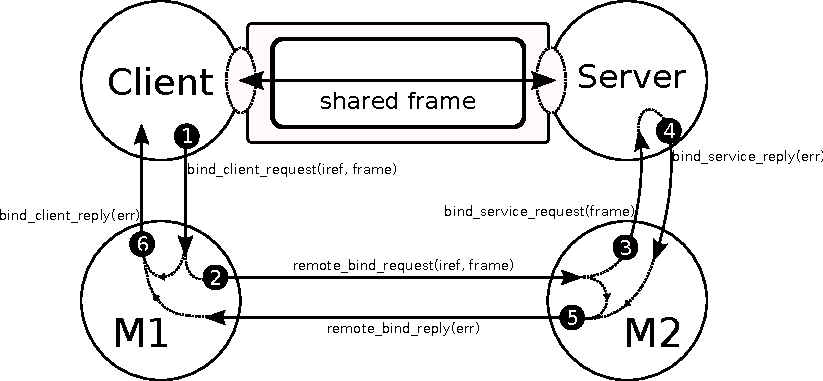
\includegraphics[width=\columnwidth]{figures/ump_bind}
  \caption{UMP bind process}\label{fig:ump_bind}
\end{figure}

Figure~\ref{fig:ump_bind} shows the steps in setting up UMP binding:
\begin{enumerate}
 \item The client sends \lstinline+bind_ump_client_request+ to its local monitor,
      with the iref, the client's (opaque) connection ID, and various parameters
      that are specific to the interconnect driver. For UMP, this includes a
      capability to a shared frame, which will be used for message transfer.
 \item The local monitor determines (from the iref) the core on which the
      service resides, and forwards the request to the monitor on that core
      using a \lstinline+bind_ump_request+ message (NB: mislabelled
      \lstinline+remote_bind_request+ in the figure).
 \item The monitor on the server's core determines the local dispatcher which
      has exported this iref, and forwards the bind request to it using a
      \lstinline+bind_ump_service_request+ message. It also provides the
      opaque service identifier which the dispatcher gave when originally
      exporting the service.
 \item The server dispatcher uses the service identifier to locate and invoke
      the connection callback for the given service. Assuming this succeeds, it
      allocates its local state for the binding (e.g. the binding object). It
      then replies to its local monitor with a
      \lstinline+bind_ump_reply_monitor+ message (labelled
      \lstinline+bind_service_reply+ in the figure).
 \item The monitor proxies the reply back to the monitor on the client's core
 \item The monitor on the client core proxies the reply back to the client,
      providing the client's connection ID, which allows it to locate the
      binding object and run the bind callback. The binding has now completed.
\end{enumerate}

The binding mechanisms for other interconnect drivers (e.g. LMP, BMP) are
similar, in that they involve an exchange of capabilities between client and
server mediated by the monitors. Once the binding is established, direct
communication can take place using the exchanged resources.

\section{Indirect capability transfer}
\label{sec:capxfer}

Because capabilities are maintained as references to per-core state in the
CPU drivers, only the LMP interconnect driver, which traverses kernel-mode
code, can directly deliver a capability along with untyped message payload.
For other interconnect drivers, such as UMP, capabilities travel out-of-band
from message payload through the monitors.

The process of indirect transmission of capabilities is as follows:
\begin{enumerate}
 \item The binding object waits to acquire a mutex on its local monitor binding.
     This is necessary, because it must send a message to its local monitor, and
     the local monitor binding is shared by all bindings (and binding-related
     code) executing on the same dispatcher. While waiting, it sends the
     non-capability payload of the message as usual.

  \item Upon receipt of the first message payload, the receiver sends back an
     acknowledgement that it is ready to receive a capability. This handshake
     is necessary to avoid over-running the receiver's buffers, and to ensure
     that capabilities can be associated with the correct messages.

  \item Once the monitor binding mutex is acquired, and the capability
     acknowledgement has been seen, a \lstinline+cap_send_request+ message
     is sent to the local monitor, containing the capability and an identifier
     for the channel on which the capability is to be sent.

  \item The monitor determines whether the cap may be sent to the remote core.
    A full discussion of the rules used is beyond the scope of this document,
    but in general capability types that refer to inherently local state (such
    as LMP endpoints) may not be sent, nor may capabilities that are currently
    being revoked. If the check fails, a \lstinline+cap_send_reply+ error is
    sent back to the local dispatcher; if it succeeds, the capability is
    serialised and proxied to the remote monitor as another
    \lstinline+cap_send_request+ message on the inter-monitor channel.

  \item The remote monitor reconstructs the capability from its serialised
    representation, and forwards it on to the destination dispatcher with a
    \lstinline+cap_receive_request+ message.

  \item The receiver identifies the binding to which the capability belongs,
    and invokes a callback on that binding. This in turn stores the capability
    in the appropriate location.

  \item When the last capability and message payload are received, the binding
   object delivers the message to the user as usual.
\end{enumerate}


\chapter{Interconnect drivers}\label{cha:icds}

\section{LMP: local (intra-core) message passing}
\label{sec:lmp_icd}

\subsection{Messaging with the local Monitor}
\label{sec:monitor}


\section{UMP: user-level message passing with coherent shared memory}
\label{sec:ump_icd}

\section{RCK: message passing on the SCC}
\label{sec:rck_icd}

\section{BMP: Beehive message passing}
\label{sec:bmp_icd}

\chapter{Additional Flounder backends}

\section{Loopback}

\section{Message buffers}

\section{RPC Client}
\label{sec:rpcclient}

\section{THC}
\label{sec:thc}

\section{AHCI Command Translator}
\label{sec:ahci}

This backend is documented in the AHCI TN.

\chapter{Name service}
\label{cha:nameservice}

TODO


\chapter{Interaction with Hake build system}
\label{cha:hake}

TODO

\begin{itemize}
 \item Configuration options
 \item Contents of Hakefiles
 \item Location/contents of generated files
 \item Dependencies
\end{itemize}


\chapter{Unsupported features and future work}

TODO

\begin{itemize}
 \item Connection/binding teardown
 \item Variable-length arrays of types other than \lstinline+char+,
        \lstinline+int8+ and \lstinline+uint8+
 \item Types shared by multiple interfaces, control over C naming of generated
        type definitions
 \item Non-blocking variant of \lstinline+get_next_event()+
 \item Fast LRPC optimisations (combines waitset, thread switch and send)
\end{itemize}

%%%%%%%%%%%%%%%%%%%%%%%%%%%%%%%%%%%%%%%%%%%%%%%%%%%%%%%%%%%%%%%%%%%%%%%%
\bibliographystyle{plain} 
\bibliography{defs,barrelfish}

\end{document}
